\documentclass[12pt,letterpaper]{article}\usepackage[]{graphicx}\usepackage[]{color}
%% maxwidth is the original width if it is less than linewidth
%% otherwise use linewidth (to make sure the graphics do not exceed the margin)
\makeatletter
\def\maxwidth{ %
  \ifdim\Gin@nat@width>\linewidth
    \linewidth
  \else
    \Gin@nat@width
  \fi
}
\makeatother

\definecolor{fgcolor}{rgb}{0.345, 0.345, 0.345}
\newcommand{\hlnum}[1]{\textcolor[rgb]{0.686,0.059,0.569}{#1}}%
\newcommand{\hlstr}[1]{\textcolor[rgb]{0.192,0.494,0.8}{#1}}%
\newcommand{\hlcom}[1]{\textcolor[rgb]{0.678,0.584,0.686}{\textit{#1}}}%
\newcommand{\hlopt}[1]{\textcolor[rgb]{0,0,0}{#1}}%
\newcommand{\hlstd}[1]{\textcolor[rgb]{0.345,0.345,0.345}{#1}}%
\newcommand{\hlkwa}[1]{\textcolor[rgb]{0.161,0.373,0.58}{\textbf{#1}}}%
\newcommand{\hlkwb}[1]{\textcolor[rgb]{0.69,0.353,0.396}{#1}}%
\newcommand{\hlkwc}[1]{\textcolor[rgb]{0.333,0.667,0.333}{#1}}%
\newcommand{\hlkwd}[1]{\textcolor[rgb]{0.737,0.353,0.396}{\textbf{#1}}}%
\let\hlipl\hlkwb

\usepackage{framed}
\makeatletter
\newenvironment{kframe}{%
 \def\at@end@of@kframe{}%
 \ifinner\ifhmode%
  \def\at@end@of@kframe{\end{minipage}}%
  \begin{minipage}{\columnwidth}%
 \fi\fi%
 \def\FrameCommand##1{\hskip\@totalleftmargin \hskip-\fboxsep
 \colorbox{shadecolor}{##1}\hskip-\fboxsep
     % There is no \\@totalrightmargin, so:
     \hskip-\linewidth \hskip-\@totalleftmargin \hskip\columnwidth}%
 \MakeFramed {\advance\hsize-\width
   \@totalleftmargin\z@ \linewidth\hsize
   \@setminipage}}%
 {\par\unskip\endMakeFramed%
 \at@end@of@kframe}
\makeatother

\definecolor{shadecolor}{rgb}{.97, .97, .97}
\definecolor{messagecolor}{rgb}{0, 0, 0}
\definecolor{warningcolor}{rgb}{1, 0, 1}
\definecolor{errorcolor}{rgb}{1, 0, 0}
\newenvironment{knitrout}{}{} % an empty environment to be redefined in TeX

\usepackage{alltt}

\usepackage{amsmath}
\usepackage{bm} % for bold math symbols
\usepackage{booktabs} % better tables
\usepackage[left=.4in,right=.2in,top=.4in,bottom=.2in]{geometry} % margins
\usepackage{caption} % for subfigures
\usepackage[T1]{fontenc} % see http://goo.gl/KXXek
\usepackage{graphicx} % obviously for graphics
\usepackage{lscape}
\usepackage{listings} % source code
\usepackage{latexsym} % MBE template for some fonts
\usepackage{mathtools} % an extension to amsmath to fix bugs
\usepackage{multirow} % column cells that span multiple rows
\usepackage{natbib} % nicer references
\usepackage{paralist} % inline lists
\usepackage[section]{placeins} % keep figures and table inside section
\usepackage{setspace} % for line spacing
\usepackage{subfig} % for subfigures
%\usepackage{subcaption} % for subfigures (can't be used with subfig)
%\usepackage{tikz}
%\usepackage{tikz-qtree}
%\usetikzlibrary{arrows}
\IfFileExists{upquote.sty}{\usepackage{upquote}}{}
\begin{document}



\begin{itemize}
\item Simulation under the null for branch-site model A
\item Symmetric (ignoring branch lengths), 8-taxon tree with one foreground branch \\
  The total tree length is 6 (3 in previous sims) and now the foreground branch is 1/10th the length of the background branches.\\
  tree: (((A\#1:0.0458015,B:0.458015):0.458015,(C:0.458015,D:0.458015):0.458015):0.458015,\\((E:0.458015,F:0.458015):0.458015,(G:0.458015,H:0.458015):0.458015):0.458015);
\item $\kappa=2.0$ $p_0=0.5$ $p_1=0.5$ $\omega_0=0$
\end{itemize}

\begin{knitrout}
\definecolor{shadecolor}{rgb}{0.969, 0.969, 0.969}\color{fgcolor}

{\centering 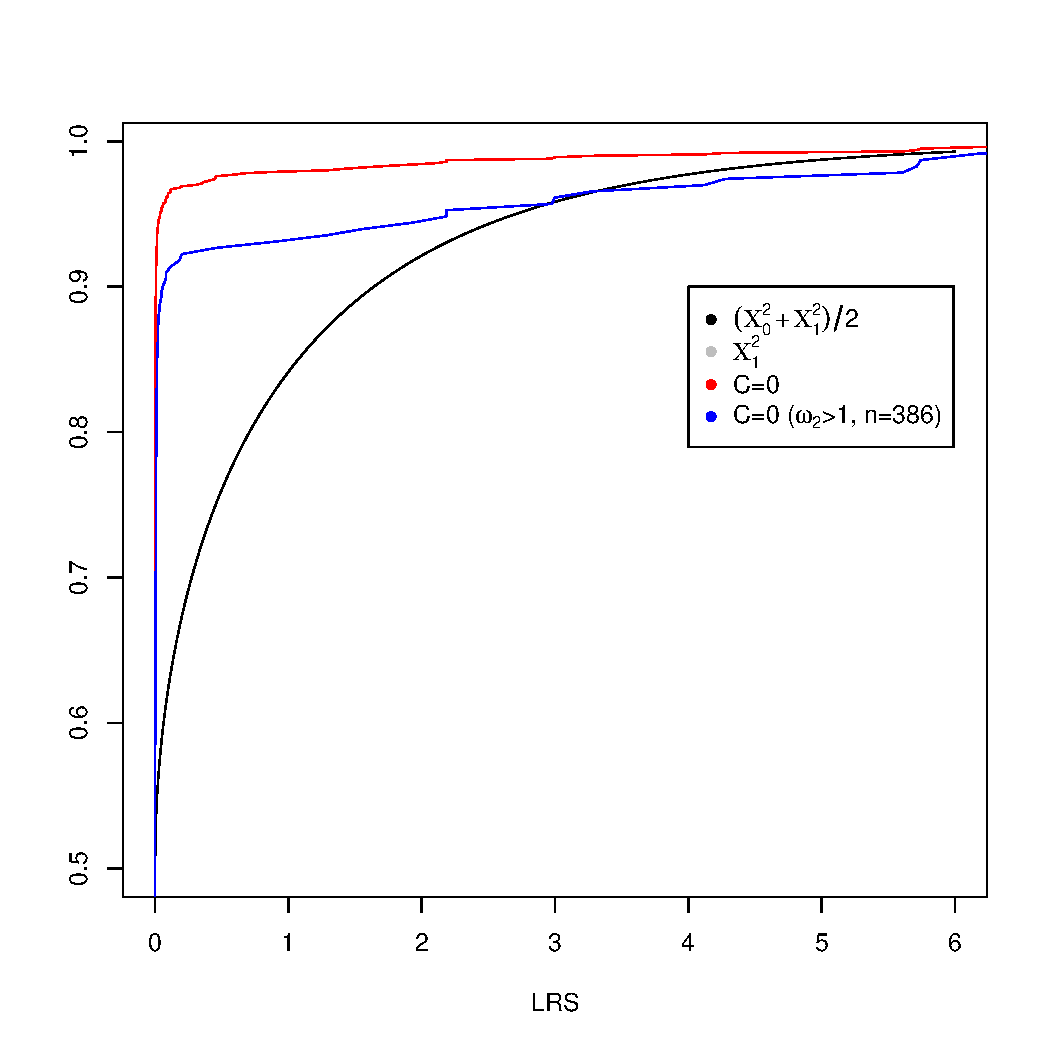
\includegraphics[width=\maxwidth]{figures/data-1} 
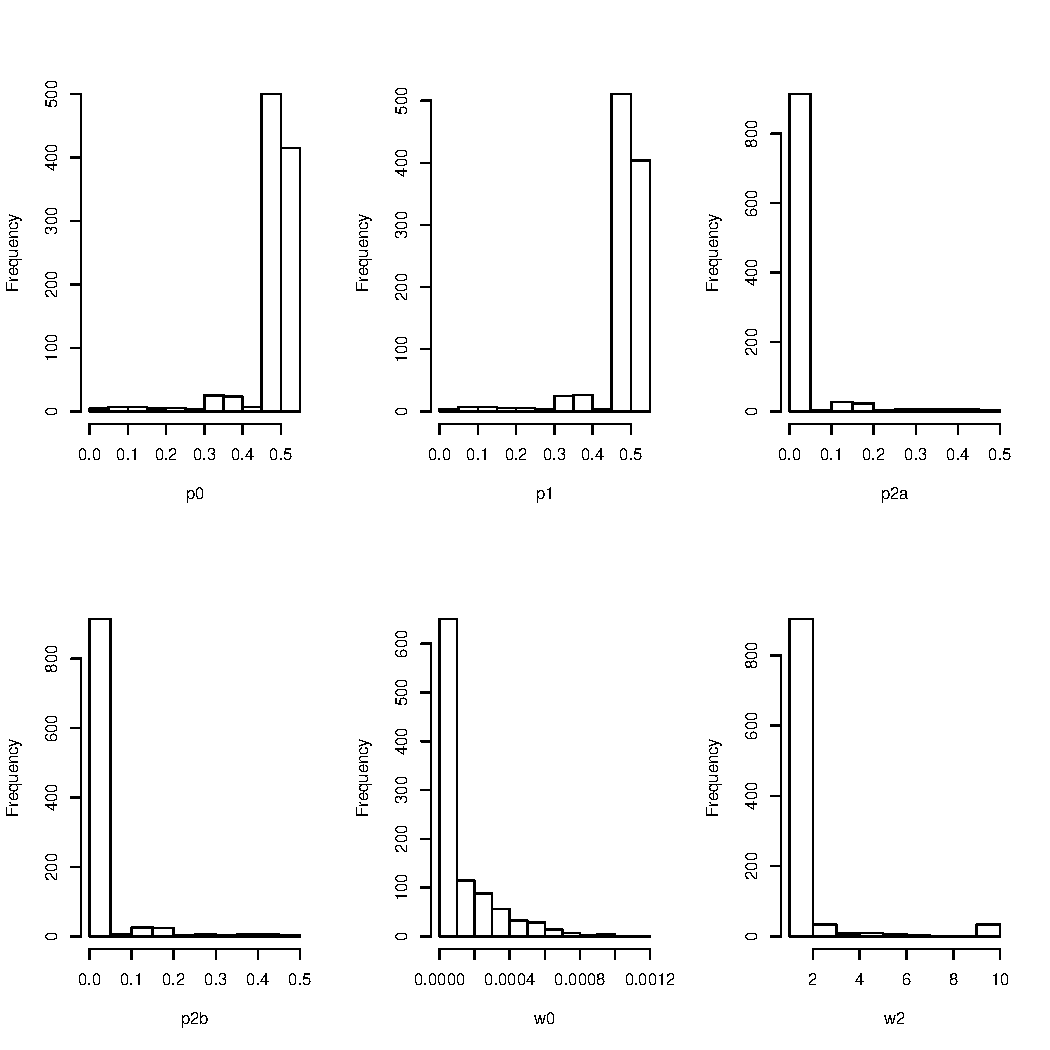
\includegraphics[width=\maxwidth]{figures/data-2} 

}



\end{knitrout}

\clearpage

These plots are for a subset of the data: $p2a>0.1$ or $p2b>0.1$.
\begin{knitrout}
\definecolor{shadecolor}{rgb}{0.969, 0.969, 0.969}\color{fgcolor}

{\centering 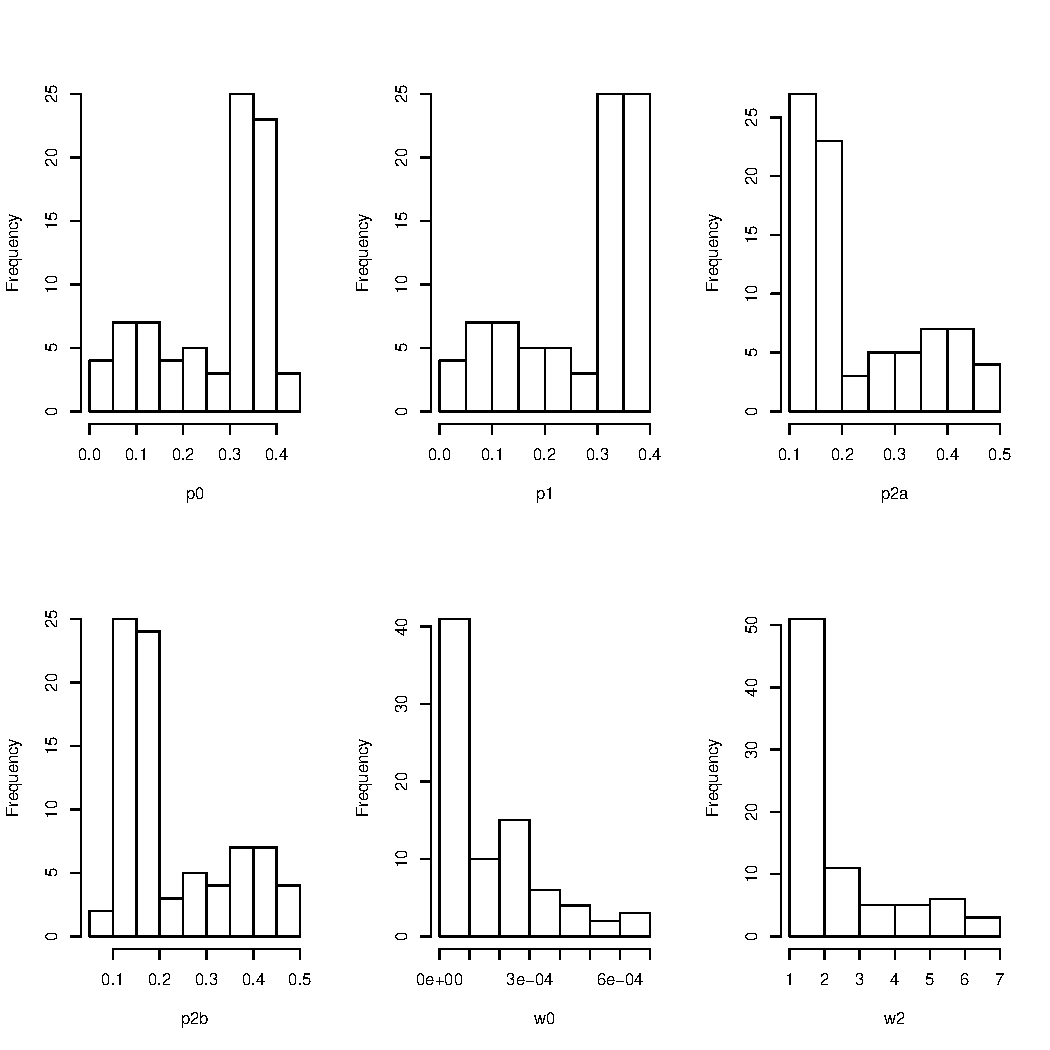
\includegraphics[width=\maxwidth]{figures/data2-1} 

}



\end{knitrout}

\clearpage

\begin{lstlisting}
> subset(params,w2>=10)
     p0      p1     p2a     p2b      w0        w2
0.50747 0.49227 0.00013 0.00013 0.00018  13.17148
0.48870 0.51093 0.00018 0.00019 0.00015 999.00000
0.50536 0.49464 0.00000 0.00000 0.00014  18.98596
0.50703 0.49296 0.00001 0.00001 0.00010  31.19575
0.50143 0.49633 0.00112 0.00111 0.00000  29.66478
0.50443 0.49555 0.00001 0.00001 0.00000  23.01739
0.50697 0.49303 0.00000 0.00000 0.00000  25.81588
0.49460 0.50540 0.00000 0.00000 0.00000  32.79931
0.50356 0.49543 0.00051 0.00050 0.00001  24.28210
0.49409 0.50588 0.00001 0.00001 0.00010  18.14854
0.50834 0.49107 0.00030 0.00029 0.00021  88.60212
0.49282 0.50643 0.00037 0.00038 0.00047  51.18785
0.49817 0.49918 0.00132 0.00132 0.00000  11.99442
0.49402 0.50556 0.00021 0.00021 0.00000  84.47536
0.49262 0.50688 0.00025 0.00025 0.00000  88.04776
0.49682 0.50233 0.00042 0.00043 0.00044  25.17260
0.49262 0.50701 0.00018 0.00019 0.00000 999.00000
0.50329 0.49504 0.00084 0.00083 0.00000  16.14985
0.50071 0.49894 0.00017 0.00017 0.00012  11.50677
0.50274 0.49725 0.00000 0.00000 0.00000  31.59949
0.49707 0.50183 0.00055 0.00055 0.00000  14.07986
0.49205 0.50784 0.00005 0.00006 0.00029  19.42556
0.49596 0.50404 0.00000 0.00000 0.00008  25.18345
0.50983 0.49017 0.00000 0.00000 0.00000  13.22519
0.50971 0.49029 0.00000 0.00000 0.00000  23.99565
0.50285 0.49618 0.00049 0.00048 0.00000  19.15881
0.49745 0.50112 0.00072 0.00072 0.00004  28.66388
0.50350 0.49596 0.00027 0.00027 0.00012  45.51805
0.50193 0.49782 0.00012 0.00012 0.00012  12.18804
0.50254 0.49746 0.00000 0.00000 0.00000  21.39871
0.49759 0.50167 0.00037 0.00037 0.00000  58.96461
0.49359 0.50550 0.00045 0.00046 0.00000  64.16664
\end{lstlisting}

\end{document}
